\documentclass[12pt]{article}
\usepackage[paper=a4paper,left=25mm,right=25mm,top=25mm,bottom=25mm]{geometry}
\usepackage[english]{babel}
\usepackage[utf8]{inputenc}
\usepackage[pdftex]{graphicx}
\usepackage{color}
\usepackage{amssymb}
\usepackage{amsthm}
\usepackage{hyperref}
\usepackage{enumitem}
\usepackage{pdfpages}
\usepackage{hyperref}


\linespread{1.25}

\begin{document}
\begin{titlepage}

\includegraphics[height=20mm]{../images/uzh_logo}\\

\begin{flushleft}

\vspace{2cm}

{\Large Introduction to Artificial Intelligence\\Exercise Sheet 9}\\

\vspace{4cm}

\textbf{Laurin van den Bergh, 16-744-401\\Yufeng Xiao, 19-763-663\\Nora Beringer, 19-734-227}\\

\vspace{2cm}

Universität Zürich\\
Institut für Informatik

\vfill Due: May 11, 2022

\vspace{3cm}


\end{flushleft}
\end{titlepage}

\newpage

\section*{Exercise 9.1}

\textbf{(a)}\\
We assume that for the population of prawns x numbers to commercialize is y $\leq$ x and number to reproduce is z = x-y.\\
The variables for $\mathbb{M}$ = $\langle$S, A, T, R, s$_{0}, \gamma \rangle$ are:\\
s$_{0}$ = 1000N\\
R(s$_{j}$, a, s$_{j}$) = 10y = 10(x-z) = 10a\\
$\gamma$ = 0.5\\
S = \{x $\mid$ x $\in$ N, 0 $\leq x \leq N$\}\\
A = \{n $\mid$ n $\in$ N, 0 $\leq n \leq N$\}\\
T(s$_{j}$, a, s$_{j}$) = 0, s$_{j}$ $<$ a\\
T(s$_{j}$, a, 2(s$_{j}$-a)) = 0.7\\
T(s$_{j}$, a, 4(s$_{j}$-a)) = 0.2\\
T(s$_{j}$, a, 0.5(s$_{j}$-a)) = 0.1\\\\
\textbf{b)} If we increase the discount factor $\gamma$ the decay will be slower for future rewards. Meaning we value future rewards more in comparison to before we increased the discount factor.\\The optimal policy changes in the regard that we sell less now and keep more N for reproduction.

\section*{Exercise 9.2}
\begin{tabular}[h]{c|c|c|c|c}
i & V$^{i}$(S$_{0}$) & V$^{i}$(S$_{1}$) & V$^{i}$(S$_{2}$) & V$^{i}$(S$_{3}$)\\
\hline
0 & 10 & 0 & 0 & 0\\
\hline
1 & 0 & 7 & 14 & 19\\
\hline
2 & 6.3 & 8.4 & 5.7 & 10\\
\hline
3 & 7.56 & 6.5 & 10.67 & 15.67\\
\hline
4 & 5.85 & 8.73 & 11.8 & 16.8\\
\hline
5 & 7.86 & 8.84 & 10.27 & 15.27\\
\end{tabular}\\\\
Like policy evaluation, value iteration formally requires an infinte numbers of iterations to converge to an exact result. We stop the iteration once the value function changes by only a small amount in a sweep. The changes do get smaller but some more iterations would be needed in order to clarify if there are still big changes coming or not.\pagebreak\\
\textbf{Policy evaluation:}\\
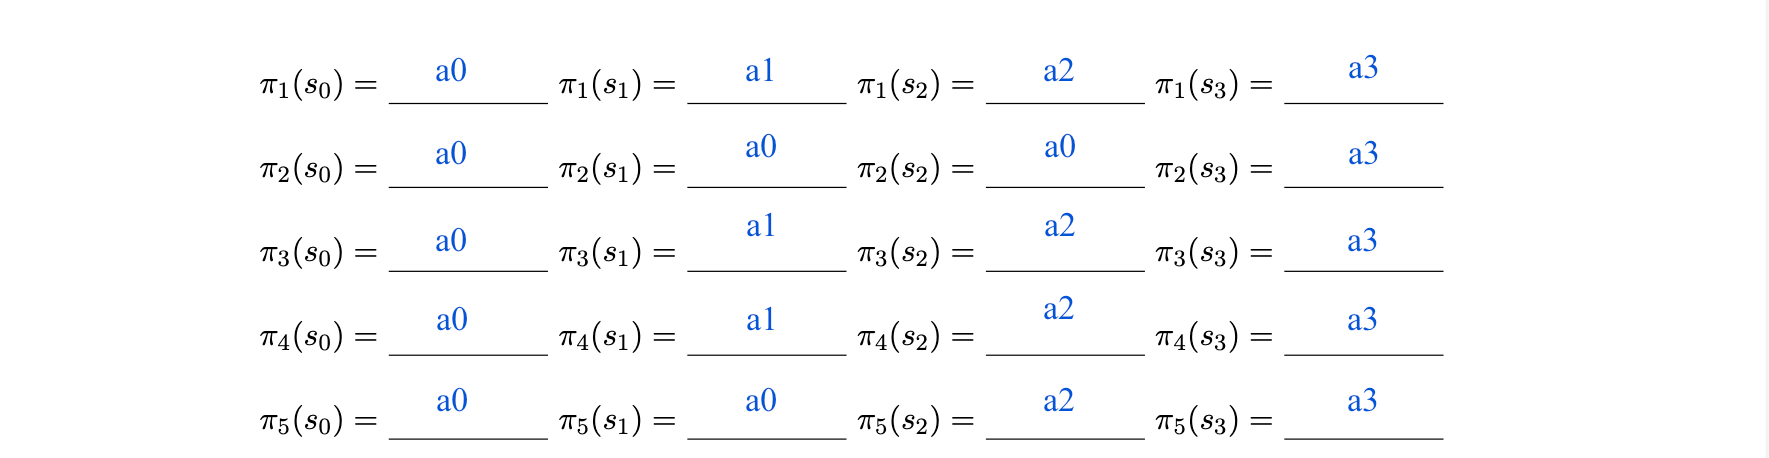
\includegraphics[scale=0.3]{9_3}




\end{document}